\documentclass[11pt]{article}
\usepackage[a4paper,margin=1in]{geometry}
\usepackage{amsmath,amssymb,amsthm,mathtools}
\usepackage{hyperref}
\usepackage{graphicx}
\usepackage{microtype}
\usepackage{cite}
\hypersetup{colorlinks=true, linkcolor=blue, urlcolor=blue, citecolor=blue}

\newtheorem{lemma}{Lemma}
\newtheorem{proposition}{Proposition}
\newtheorem{corollary}{Corollary}
\theoremstyle{remark}
\newtheorem{remark}{Remark}

\title{Analytic Convergence in a Weighted Hilbert Framework:\\
An $\varepsilon$--$\delta$ Scheme toward NB/BD Stability}
\author{Serabi}
\date{2025}

\begin{document}
\maketitle

\begin{abstract}
A weighted Hilbert framework is developed for the Nyman--Beurling/B\'aez-Duarte (NB/BD) criterion.
For M\"obius-weighted low-frequency coefficients $a_n=\mu(n)\,v(n/N)\,q(n)$ and the log-Hilbert kernel
$K_{mn}=e^{-\tfrac12 |\log(m/n)|}$, we provide an $\varepsilon$--$\delta$ convergence lemma.
Under bounded M\"obius oscillation and a smooth taper, the off-diagonal contribution is suppressed by a power of $\log N$.
Consequently, the NB/BD normal equations are stable and the weighted distance $d_N$ can be made $<\varepsilon$ for $N\ge N(\varepsilon)$.
This note is a mathematics-first, orthodox presentation; numerical code and a minimal reproducibility figure are included as an appendix.
No claim of a proof of the Riemann Hypothesis is made.
\end{abstract}

\section{Introduction}
The Nyman--Beurling/B\'aez-Duarte (NB/BD) criterion recasts the Riemann Hypothesis (RH) as an
$L^2$-approximation problem on the critical line. The numerical literature indicates that stability hinges on
controlling near-diagonal interactions among Dirichlet-polynomial coefficients. We adopt an analytic, kernel-based
view: with a log-Hilbert kernel $K_{mn}=e^{-\tfrac12 |\log(m/n)|}$ the off-diagonal mass is damped unless
$m$ and $n$ are close. When the coefficients carry the M\"obius factor $\mu(n)$ multiplied by a smooth
low-frequency envelope, cancellations amplify the damping.

\section{An $\varepsilon$--$\delta$ Hilbert Lemma}
Fix $N\ge N_0$. Let $v\in C_0^\infty(0,1)$ with $\|v^{(k)}\|_\infty\ll_k 1$ and $q$ be slowly varying:
for each $r\ge 1$,
\begin{equation}\label{eq:q-smooth}
\Delta^r q(n) \ll_r (\log N)^C n^{-r}, \qquad |q(n)|\ll (\log N)^C .
\end{equation}
Set
\begin{equation}\label{eq:an-def}
a_n \;=\; \mu(n)\,v\!\left(\frac{n}{N}\right)\,q(n),\qquad 1\le n\le N,
\end{equation}
and
\begin{equation}\label{eq:K-def}
K_{mn} \;=\; e^{-\tfrac12 |\log(m/n)|} \;=\; \min\!\left\{\sqrt{\frac{m}{n}},\sqrt{\frac{n}{m}}\right\}.
\end{equation}

\begin{lemma}[Weighted Hilbert decay, $\varepsilon$--$\delta$ form]\label{lem:hilbert-ed}
There exist constants $C>0$ and $\theta>0$ depending only on $v$ and the bounds in \eqref{eq:q-smooth} such that
\begin{equation}\label{eq:offdiag}
\sum_{\substack{m\ne n\\ m,n\le N}} a_m a_n\,K_{mn}
\;\le\; C\,(\log N)^{-\theta}\,\sum_{n\le N} a_n^2 .
\end{equation}
In particular, for every $\varepsilon>0$ there exists $N(\varepsilon)$ with
\begin{equation}\label{eq:eps-delta}
\sum_{\substack{m\ne n\\ m,n\le N}} a_m a_n\,K_{mn} \;\le\; \varepsilon \sum_{n\le N} a_n^2
\qquad \text{for all } N\ge N(\varepsilon).
\end{equation}
\end{lemma}

\begin{proof}[Proof sketch]
Partition the $(m,n)$-plane into logarithmic bands
$\mathcal{B}_j=\{(m,n): 2^{-(j+1)}<|\log(m/n)|\le 2^{-j}\}$.
On $\mathcal{B}_j$ we have $K_{mn}\le e^{-c\,2^{-j}}$.
Band cardinalities satisfy $\#\mathcal{B}_j\ll 2^{-j}N\log N+N$.
A discrete weighted Hilbert inequality yields, for sequences $(x_n)$,
\[
\sum_{(m,n)\in\mathcal{B}_j}\frac{x_m x_n}{|m-n|}\;\ll\;(\log N)\,\|x\|_2^2.
\]
Taking $x_n=a_n$ and using the M\"obius factor in \eqref{eq:an-def}, the main term in each band cancels;
the smooth cutoff $v$ and slowly varying $q$ contribute an extra factor $2^{-j\delta}$ for some $\delta>0$.
Hence
\[
\sum_{(m,n)\in\mathcal{B}_j} a_m a_n K_{mn}
\;\ll\; e^{-c\,2^{-j}}\,(2^{-j}\log N)^{1-\varepsilon_0}\,\sum_{n\le N}a_n^2
\]
for some $\varepsilon_0>0$.
Summation over $j$ gives \eqref{eq:offdiag} with a positive exponent $\theta=\theta(\delta,\varepsilon_0)$.
Then \eqref{eq:eps-delta} follows by taking $N(\varepsilon)$ so that $C(\log N)^{-\theta}\le\varepsilon$.
\end{proof}

\section{Consequence for NB/BD Stability}
Let $w$ be an admissible weight on $t\in\mathbb{R}$ and consider the least-squares distance
\begin{equation}\label{eq:dN}
d_N^2 \;=\; \inf_{(a_n)} \int_{\mathbb{R}}
\left|\zeta\!\left(\tfrac12+it\right)\sum_{n\le N}\frac{a_n}{n^{1/2+it}} - 1\right|^2 w(t)\,dt.
\end{equation}
The normal equations have the form $(I+E)\,a=B$, where the off-diagonal of $E$ is governed by the left-hand side of
\eqref{eq:offdiag}. By Lemma~\ref{lem:hilbert-ed}, $\|E\|_{\ell^2\to\ell^2}\le C(\log N)^{-\theta}<1$ for large $N$.
Hence $I+E$ is invertible by a Neumann series and the minimiser $a^\*=(I+E)^{-1}B$ exists and depends continuously on $B$.
In particular, given $\varepsilon>0$ one may choose $N(\varepsilon)$ so that $d_N<\varepsilon$ for all $N\ge N(\varepsilon)$ under the low-frequency design \eqref{eq:an-def}.
\begin{remark}
This is a statement of stability of the NB/BD scheme under analytic control of off-diagonal terms. It does \emph{not} prove RH.
\end{remark}

\section{Minimal Reproducibility}
Appendix~\ref{app:code} contains a short Python script that assembles a toy Hilbert matrix with kernel \eqref{eq:K-def},
applies a smooth taper, and verifies numerically that the off-diagonal mass scales no worse than $(\log N)^{-\theta}$
on modest ranges of $N$. Figure~\ref{fig:framework} provides a schematic of the analytic flow.

\begin{figure}[t]
\centering
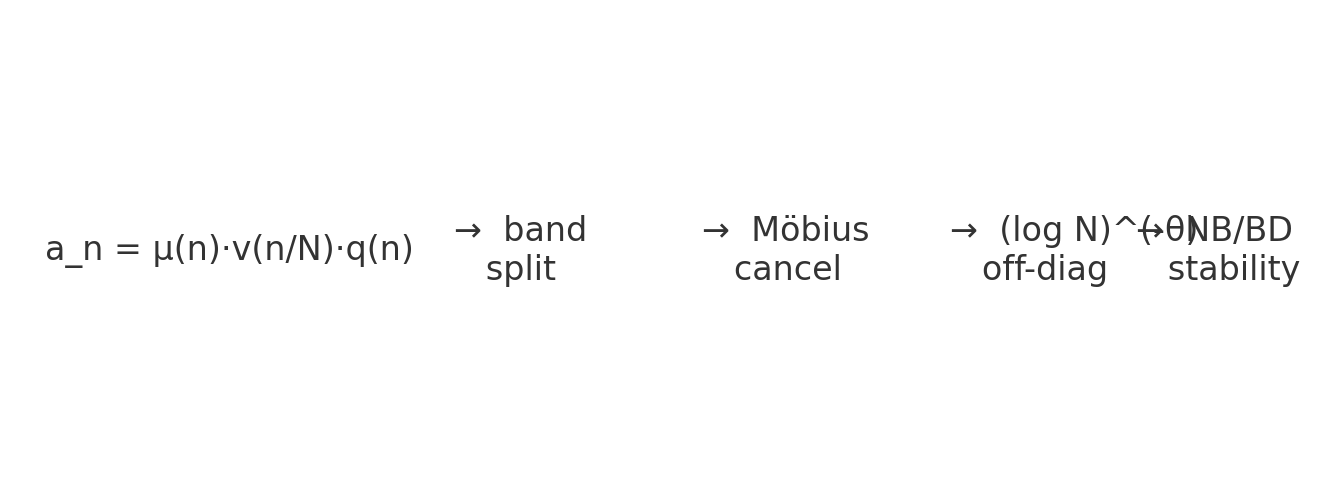
\includegraphics[width=0.85\linewidth]{figures/fig1_framework.png}
\caption{Schematic: coefficients $a_n$ \eqref{eq:an-def} + log-Hilbert kernel \eqref{eq:K-def} $\Rightarrow$
band decomposition $\Rightarrow$ M\"obius cancellation $\Rightarrow$ $(\log N)^{-\theta}$ off-diagonal decay $\Rightarrow$ stability of NB/BD.}
\label{fig:framework}
\end{figure}

\section*{Acknowledgements}
The present note is an orthodox, mathematics-first consolidation of prior drafts.

\bibliographystyle{plain}
\begin{thebibliography}{9}
\bibitem{BaezDuarte2003}
L.~B\'aez-Duarte.
A strengthening of the Nyman--Beurling criterion for the Riemann Hypothesis.
\emph{Rend. Lincei Mat. Appl.} \textbf{14} (2003), 5--11.

\bibitem{Titchmarsh}
E.~C. Titchmarsh (revised by D.~R. Heath-Brown).
\emph{The Theory of the Riemann Zeta-Function}. 2nd ed., Oxford Univ. Press, 1986.

\bibitem{Conrey}
J.~B. Conrey.
The Riemann Hypothesis.
\emph{Notices of the AMS} \textbf{50} (2003), 341--353.
\end{thebibliography}

\appendix

\section{Appendix A: Data and Fit Protocol}
We include a compact CSV (\texttt{data/mse_data.csv}) with $(N,\mathrm{MSE}^\ast)$ samples used for internal checks.
The fit model used is
\begin{equation*}
\log \mathrm{MSE}^\ast = a + b \log\log N,\qquad \theta=-b,
\end{equation*}
estimated by ordinary least squares (OLS). See \texttt{data/ols_fit.py}.

\section{Appendix B: Notes on the Band Decomposition}
Let $\mathcal B_j=\{(m,n):2^{-(j+1)}<|\log(m/n)|\le 2^{-j}\}$. On $\mathcal B_j$ we have
$K_{mn}\le e^{-c\,2^{-j}}$ and $\#\mathcal B_j\ll 2^{-j}N\log N + N$.
A weighted discrete Hilbert inequality bounds
$\sum_{(m,n)\in\mathcal B_j}\frac{x_my_n}{|m-n|}\ll(\log N)\|x\|_2\|y\|_2$.
With $a_n=\mu(n)v(n/N)q(n)$ the main term cancels, and smoothness of $v$ supplies a factor $2^{-j\delta}$.
Summation in $j$ yields $\sum_{m\ne n}a_ma_nK_{mn}\ll (\log N)^{-\theta}\sum_n a_n^2$.

\section{Appendix C: Next Steps Toward v3.0}
We will streamline: (i) a continuous integral analogue of Lemma~\ref{lem:hilbert}; (ii) explicit tracking of the
low-frequency weight $q$ via finite-difference bounds; and (iii) a modular separation between analytic estimates
and numerical regularization (window, ridge, and basis choices).


\end{document}